\documentclass[14pt]{extbook}
\usepackage{multicol, enumerate, enumitem, hyperref, color, soul, setspace, parskip, fancyhdr} %General Packages
\usepackage{amssymb, amsthm, amsmath, bbm, latexsym, units, mathtools} %Math Packages
\everymath{\displaystyle} %All math in Display Style
% Packages with additional options
\usepackage[headsep=0.5cm,headheight=12pt, left=1 in,right= 1 in,top= 1 in,bottom= 1 in]{geometry}
\usepackage[usenames,dvipsnames]{xcolor}
\usepackage{dashrule}  % Package to use the command below to create lines between items
\newcommand{\litem}[1]{\item#1\hspace*{-1cm}\rule{\textwidth}{0.4pt}}
\pagestyle{fancy}
\lhead{Progress Quiz 8}
\chead{}
\rhead{Version C}
\lfoot{4553-3922}
\cfoot{}
\rfoot{Fall 2020}
\begin{document}

\begin{enumerate}
\litem{
Determine the horizontal and/or oblique asymptotes in the rational function below.\[ f(x) = \frac{12x^{3} +43 x^{2} +51 x + 20}{4x^{2} +25 x + 25} \]\begin{enumerate}[label=\Alph*.]
\item \( \text{Horizontal Asymptote of } y = 3.000  \)
\item \( \text{Horizontal Asymptote of } y = 3.000 \text{ and Oblique Asymptote of } y = 3x -8 \)
\item \( \text{Horizontal Asymptote at } y = -5.000 \)
\item \( \text{Oblique Asymptote of } y = 3x -8. \)
\item \( \text{Horizontal Asymptote of } y = 0 \)

\end{enumerate} }
\litem{
Which of the following functions \textit{could} be the graph below?
\begin{center}
    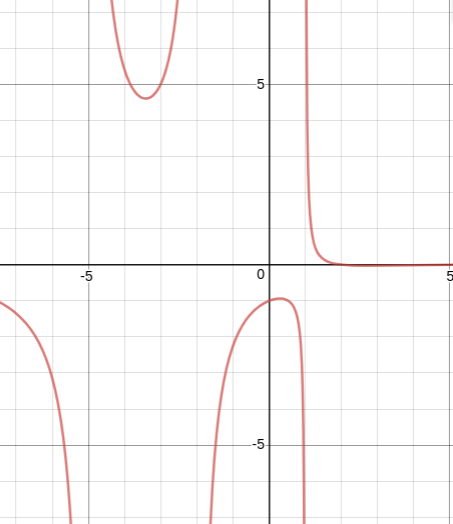
\includegraphics[width=0.5\textwidth]{../Figures/identifyGraphOfRationalFunctionCopyC.png}
\end{center}
\begin{enumerate}[label=\Alph*.]
\item \( f(x)=\frac{x^{3} -2 x^{2} -7 x -4}{x^{3} +5 x^{2} -26 x -120} \)
\item \( f(x)=\frac{x^{3} -11 x^{2} +34 x -24}{x^{3} -5 x^{2} -26 x + 120} \)
\item \( f(x)=\frac{x^{3} +11 x^{2} +34 x + 24}{x^{3} +5 x^{2} -26 x -120} \)
\item \( f(x)=\frac{x^{3} -11 x^{2} +34 x -24}{x^{3} -5 x^{2} -26 x + 120} \)
\item \( \text{None of the above are possible equations for the graph.} \)

\end{enumerate} }
\litem{
Determine the vertical asymptotes and holes in the rational function below.\[ f(x) = \frac{12x^{3} +41 x^{2} -10 x -75}{12x^{2} +29 x + 15} \]\begin{enumerate}[label=\Alph*.]
\item \( \text{Holes at } x = -0.75 \text{ and } x = -1.667 \text{ with no vertical asymptotes.} \)
\item \( \text{Vertical Asymptote of } x = -0.75 \text{ and hole at } x = -1.667 \)
\item \( \text{Vertical Asymptote of } x = 1.0 \text{ and hole at } x = -1.667 \)
\item \( \text{Vertical Asymptotes of } x = -0.75 \text{ and } x = -1.667 \text{ with no holes.} \)
\item \( \text{Vertical Asymptotes of } x = -0.75 \text{ and } x = 1.25 \text{ with a hole at } x = -1.667 \)

\end{enumerate} }
\litem{
Determine the vertical asymptotes and holes in the rational function below.\[ f(x) = \frac{12x^{3} -41 x^{2} -40 x + 48}{9x^{2} +18 x + 8} \]\begin{enumerate}[label=\Alph*.]
\item \( \text{Vertical Asymptote of } x = 1.333 \text{ and hole at } x = -1.333 \)
\item \( \text{Vertical Asymptotes of } x = -0.667 \text{ and } x = 0.75 \text{ with a hole at } x = -1.333 \)
\item \( \text{Vertical Asymptotes of } x = -0.667 \text{ and } x = -1.333 \text{ with no holes.} \)
\item \( \text{Holes at } x = -0.667 \text{ and } x = -1.333 \text{ with no vertical asymptotes.} \)
\item \( \text{Vertical Asymptote of } x = -0.667 \text{ and hole at } x = -1.333 \)

\end{enumerate} }
\litem{
Determine the horizontal and/or oblique asymptotes in the rational function below.\[ f(x) = \frac{16x^{3} +48 x^{2} -25 x -75}{4x^{2} -17 x + 15} \]\begin{enumerate}[label=\Alph*.]
\item \( \text{Horizontal Asymptote of } y = 4.0  \)
\item \( \text{Horizontal Asymptote of } y = 4.0 \text{ and Oblique Asymptote of } y = 4x + 29 \)
\item \( \text{Horizontal Asymptote at } y = 3.0 \)
\item \( \text{Oblique Asymptote of } y = 4x + 29. \)
\item \( \text{Horizontal Asymptote of } y = 3.0 \text{ and Oblique Asymptote of } y = 4x + 29 \)

\end{enumerate} }
\litem{
Determine the horizontal and/or oblique asymptotes in the rational function below.\[ f(x) = \frac{9x^{3} -48 x^{2} +73 x -30}{3x^{2} -17 x + 10} \]\begin{enumerate}[label=\Alph*.]
\item \( \text{Horizontal Asymptote of } y = 3.0  \)
\item \( \text{Horizontal Asymptote of } y = 3.0 \text{ and Oblique Asymptote of } y = 3x + 1 \)
\item \( \text{Horizontal Asymptote of } y = 5.0 \text{ and Oblique Asymptote of } y = 3x + 1 \)
\item \( \text{Oblique Asymptote of } y = 3x + 1. \)
\item \( \text{Horizontal Asymptote at } y = 5.0 \)

\end{enumerate} }
\litem{
Which of the following functions \textit{could} be the graph below?
\begin{center}
    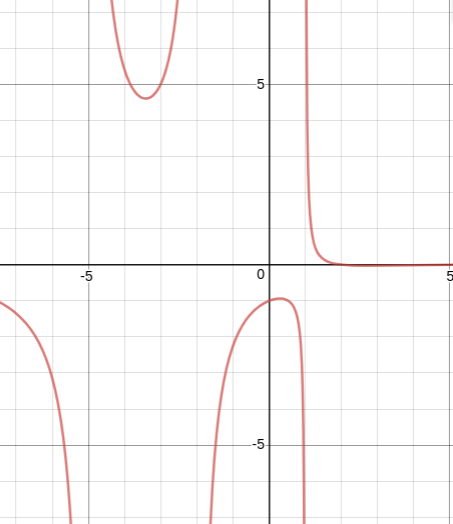
\includegraphics[width=0.5\textwidth]{../Figures/identifyGraphOfRationalFunctionC.png}
\end{center}
\begin{enumerate}[label=\Alph*.]
\item \( f(x)=\frac{x^{3} -3 x^{2} -13 x + 15}{x^{3} +4 x^{2} -15 x -18} \)
\item \( f(x)=\frac{x^{3} -1 x^{2} -9 x + 9}{x^{3} -4 x^{2} -15 x + 18} \)
\item \( f(x)=\frac{x^{3} + x^{2} -9 x -9}{x^{3} +4 x^{2} -15 x -18} \)
\item \( f(x)=\frac{x^{3} -1 x^{2} -9 x + 9}{x^{3} -4 x^{2} -15 x + 18} \)
\item \( \text{None of the above are possible equations for the graph.} \)

\end{enumerate} }
\litem{
Determine the vertical asymptotes and holes in the rational function below.\[ f(x) = \frac{6x^{3} -11 x^{2} -x + 6}{4x^{2} -16 x + 15} \]\begin{enumerate}[label=\Alph*.]
\item \( \text{Holes at } x = 2.5 \text{ and } x = 1.5 \text{ with no vertical asymptotes.} \)
\item \( \text{Vertical Asymptote of } x = 2.5 \text{ and hole at } x = 1.5 \)
\item \( \text{Vertical Asymptote of } x = 1.5 \text{ and hole at } x = 1.5 \)
\item \( \text{Vertical Asymptotes of } x = 2.5 \text{ and } x = 1.5 \text{ with no holes.} \)
\item \( \text{Vertical Asymptotes of } x = 2.5 \text{ and } x = -0.667 \text{ with a hole at } x = 1.5 \)

\end{enumerate} }
\litem{
Determine the vertical asymptotes and holes in the rational function below.\[ f(x) = \frac{6x^{3} + x^{2} -39 x + 36}{9x^{2} -18 x + 8} \]\begin{enumerate}[label=\Alph*.]
\item \( \text{Vertical Asymptotes of } x = 0.667 \text{ and } x = 1.5 \text{ with a hole at } x = 1.333 \)
\item \( \text{Holes at } x = 0.667 \text{ and } x = 1.333 \text{ with no vertical asymptotes.} \)
\item \( \text{Vertical Asymptote of } x = 0.667 \text{ and hole at } x = 1.333 \)
\item \( \text{Vertical Asymptotes of } x = 0.667 \text{ and } x = 1.333 \text{ with no holes.} \)
\item \( \text{Vertical Asymptote of } x = 0.667 \text{ and hole at } x = 1.333 \)

\end{enumerate} }
\litem{
Determine the horizontal and/or oblique asymptotes in the rational function below.\[ f(x) = \frac{10x^{3} +39 x^{2} +44 x + 12}{5x^{2} -13 x -6} \]\begin{enumerate}[label=\Alph*.]
\item \( \text{Horizontal Asymptote at } y = 3.000 \)
\item \( \text{Horizontal Asymptote of } y = 0 \)
\item \( \text{Horizontal Asymptote of } y = 2.000  \)
\item \( \text{Oblique Asymptote of } y = 2x + 13. \)
\item \( \text{Horizontal Asymptote of } y = 2.000 \text{ and Oblique Asymptote of } y = 2x + 13 \)

\end{enumerate} }
\end{enumerate}

\end{document}